\documentclass[fleqn,10pt]{physiome}
% Use option lineno for line numbers 
\usepackage{tabularx}

\articletype{Original}
%% Choose from Original, Retrospective, Review, Letter

\title{A Quantitative Model of Human Jejunal Smooth Muscle Cell Electrophysiology}

\author[1][weiwei.ai@auckland.ac.nz]{Weiwei Ai}
\author[1]{David P Nickerson}
\affil[1]{Auckland Bioengineering Institute, University of Auckland, New Zealand}



%% The following lines can be omitted when submitting;
%% information will be added by editors
\publicationdate{30 July 2021}
\editor{Shelley Fong}
\curator{Anand Rampadarath}
\submitteddate{09 Aug 2021}
\accepteddate{09 Sept 2021}
\citethisas{Ai and Nickerson (2020)\\A Quantitative Model of Human Jejunal Smooth Muscle Cell Electrophysiology. Physiome. }{10.36903/physiome.16590317}


\begin{document}
\maketitle

\begin{abstract}
The \citet{poh2012quantitative} paper describes the first biophysically based computational model of human jejunal smooth muscle cell (hJSMC) electrophysiology. The ionic currents are described by either a traditional Hodgkin-Huxley (HH) formalism or a deterministic multi-state Markov (MM) formalism. We create a modularized CellML implementation of the model, which is able to reproduce clamping behaviours of individual currents and whole cell action potential traces. In addition, some inconsistencies have been uncovered and discussed in this paper.
\end{abstract}

\keywords{Human jejunal smooth muscle cell, computational model, CellML}

\primarypubs[10.36903/physiome.16590317]{sample}{poh2012quantitative}

\section{Introduction}

In the primary paper \citep{poh2012quantitative}, the first biophysically based model of human jejunal smooth muscle cell (hJSMC) electrophysiology was presented. Here, we divide the mathematical model into distinct sub-modules encoded in CellML enabling reuse of the various sub-modules in future studies and models. We attempt to reproduce individual ionic currents, cellular voltage behaviour and sensitive analysis corresponding to changes of channel conductance. From the primary paper we extracted data using the Engauge digitizer software \citep{mitchell_markummitchellengauge-digitizer_2020} to compare the current simulation results against those in the primary publication. In doing so, we found inconsistencies in parameter values and mathematical equations presented in the primary paper, as well as the simulation experiment settings. These discrepancies are discussed in \autoref{sec:discussion}.

\section{Model description}
\label{sed:modelDescription}

\subsection{Primary Publication}

In the hJSMC model \citep{poh2012quantitative}, L-type calcium channels, the large conductance calcium and voltage activated potassium channels (BK) channels, and sodium channels are formulated using a deterministic multi-state Markov (MM) model \citep{19961078}, while the T-type calcium channels and voltage dependent potassium current employ a traditional Hodgkin-Huxley (HH) formalism \citep{hodgkin1952quantitative}. The sodium calcium exchanger and sodium potassium pump formulation are based on the work proposed by \citet{ten2004model}. The primary publication shows that the model has been validated against a wide range of experiments and data. The authors also provide CellML code \url{https://models.physiomeproject.org/w/yc_poh/poh_2012} and C code \url{https://computationalbiolab.github.io/jejunal_smc_model/}. The mathematical descriptions in the publication \citep{poh2012quantitative} along with these codes are the basis to build the curated CellML implementation presented here.

\subsection{Modularized CellML model}
The modularized version of the CellML implementation is available on Physiome Model Repository (PMR) at \url{https://models.physiomeproject.org/workspace/692} and the documentation can be found in the corresponding exposure at \url{https://models.physiomeproject.org/e/6c7}. In this manuscript we focus on reproducibility and reusability. The main components of this model and the performed simulation experiments are summarized as follows.

The \emph{membrane potential component} defines the complete equations of the membrane potential and total ionic current. It combines the imported ionic current components and ionic concentrations components. The component can be stimulated by various periodic stimuli and generates a sequence of action potentials. The \emph{clamped current component} defines the complete equations of the total and individual ionic currents, when performing voltage or concentration clamp simulation experiments.

The individual \emph{ionic current components} share the same formulation $I=g_{max}PO(V_m-E)$, where $V_m$ is the membrane potential and $E=\dfrac{RT}{zF}ln\left(\dfrac{X_o}{X_i} \right)$ is the reversal potential defined in the \emph{Nernst potential component}. The open probability $PO$ computation depends on the formalism. For L-type calcium channels, the large conductance calcium and voltage activated potassium channels (BK) channels, sodium channels, a deterministic multi-state Markov (MM) model \citep{19961078} is used to describe various channel states. Such currents incorporate the \emph{channel states} components. The Hodgkin-Huxley (HH) formalism of the T-type calcium channels and voltage dependent potassium current includes the \emph{gating kinetics} components along with steady state of gates and time constants components. The sodium calcium exchanger and sodium potassium pump formulation is different from the aforementioned currents, which is defined in its own component.

The \emph{ionic concentrations component} defines the dependence of the intracellular concentrations on the membrane currents. The  \emph{temperature factor component} encodes the temperature coefficient $\phi=Q_{10}^{\frac{T-T_0}{10}}$, where $Q_{10}$ is species specific parameter, $T_{0}$ is the reference temperature (i.e., the model construction temperature), and $T$ is the desired temperature for a given simulation experiment. This coefficient is included in the equations listed in \autoref{tab:equations}.

Following best practices, our CellML implementation separates the mathematics from the parameterisation of the model. The mathematical model is imported into a specific parameterised instance in order to perform numerical simulations. The parameterisation would include defining the stimulus protocol to be applied. We have three sets of simulation experiments and corresponding simulation results to reproduce the corresponding figures in the primary publication: 
\begin{enumerate}[noitemsep] 
\item the \emph{patch clamp experiment} is used to validate the individual ionic currents;
\item the \emph{periodic stimulation experiment} is used to generate a sequence of action potentials; and
\item the \emph{sensitivity analysis experiment} is used to evaluate the contributions of currents to the membrane voltage.
\end{enumerate}

Simulation settings and detailed solver information are encoded in SED-ML documents for execution of the simulation experiments \citep{waltemath_reproducible_2011}. The Python scripts used with OpenCOR \citep{garny_opencor_2015} to perform simulations and produce the figures in the primary paper are also included in the folder \texttt{<Simulation>}. The name of the simulation and plot scripts indicate the figure number in the primary paper. For example, \texttt{Fig2\_sim.py} is used to generate the simulation data and \texttt{Fig2\_plot.py} reproduces the graph shown in Figure 2 from \citet{poh2012quantitative}.

\section{Model results}
\label{sed:modelResults}

\subsection{Response of individual ionic currents to clamped voltage}
In the \emph{patch clamp experiment}, the \emph{clamped current component} is configured and parameterised with an applied \emph{patch clamp protocol}. The clamping parameters can be changed by the user, while the values used in this article are listed in \autoref{tab:clamp}. The holding voltage duration is $1$ second and the temperature is $297$ Kelvin. The simulation experiment can be performed by loading the corresponding SED-ML document into OpenCOR and executing the simulation. By increasing the intracellular concentrations, we have reproduced the IV curves in Figures \ref{simFig2}, \ref{simFig3} and \ref{simFig6}, however, the specific experiment settings cannot be confirmed by the authors.

\begin{table}[hbt!]\centering
\caption{Clamping parameters}\label{tab:clamp}
\resizebox{\textwidth}{!} {
\begin{tabular}{ccccc}
\toprule
Fig & Holding voltage (mV) & Test voltages (mV) &  Current& $X_i$(mM)\\
\midrule
2 & -100 & -90:5:40  & $I_{CaL}$ & $Ca_{i}^{2+}=5.388e-5$ ,$Ca_{i}^{2+}=0.11$ \\
3 & -100 & -90:5:40 & $I_{CaT}$ & $Ca_{i}^{2+}=5.388e-5$ ,$Ca_{i}^{2+}=0.11$ \\
4 & -70 & -70:5:-15 & $I_{Kv}$ & $K_{i}^{+}=153.6$ \\
5 & -70 & -70:10:70  & $I_{BK}$ & $K_{i}^{+}=153.6$, $Ca_{i}^{2+}=0.001$, $Ca_{i}^{2+}=0.0003$ \\
6 & -100 & -90:5:30  & $I_{Na}$ & $Na_{i}^{+}=10.57$, $Na_{i}^{+}=50$ \\
\bottomrule
\end{tabular}
}
\end{table}

In the presented figures, the dots denote the simulated data extracted from the primary publication, while the solid lines are the simulation results produced by the current CellML implementation.

\autoref{simFig2} shows the normalized L-type $Ca^{2+}$ channels peak I–V plot with different intracelluar concentrations. During simulation, the $\theta$ and $\delta$ in Equations S-33 and S-34 are set to 0 to switch off the $Ca_i^{2+}$ dependency. \autoref{simFig3} shows normalized T-type $Ca^{2+}$ channels peak I–V plot.


\begin{figure}
\centering
\begin{minipage}{.5\textwidth}
  \centering
  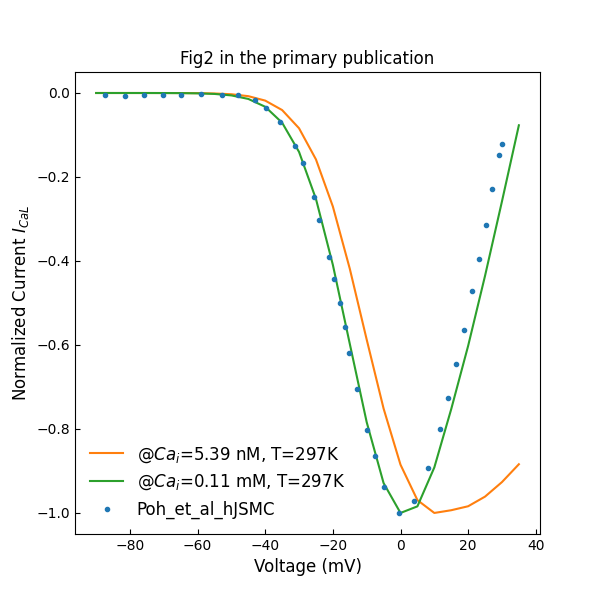
\includegraphics[width=\linewidth]{./figs/simFig2.png}
  \captionof{figure}{Normalized L-type $Ca^{2+}$ channels peak I–V plot (\emph{c.f.,} Fig.~2 in \citet{poh2012quantitative}).}
  \label{simFig2}
\end{minipage}%
\begin{minipage}{.5\textwidth}
  \centering
  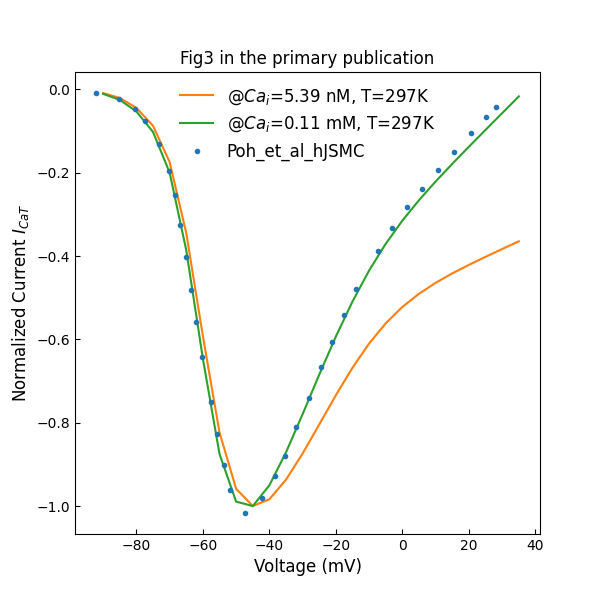
\includegraphics[width=\linewidth]{./figs/simFig3.png}
  \captionof{figure}{Normalized T-type $Ca^{2+}$ channels peak I–V plot  (\emph{c.f.,} Fig.~3 in \citet{poh2012quantitative}).}
  \label{simFig3}
\end{minipage}
\end{figure}

\autoref{simFig4} shows normalized I–V plot of whole cell voltage-activated potassium currents. The holding voltage was not specified in the primary paper, and we assume here a value of $-70$ mV.

\begin{figure}
\centering
\begin{minipage}{.5\textwidth}
  \centering
  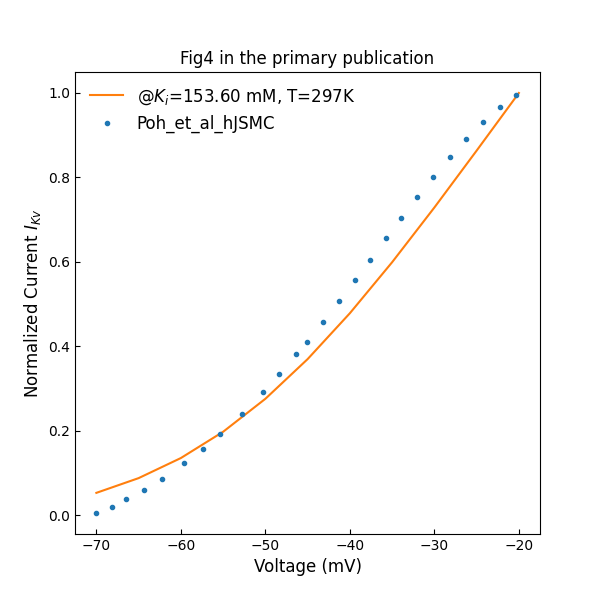
\includegraphics[width=\linewidth]{./figs/simFig4.png}
  \captionof{figure}{Normalized I–V plot of whole cell voltage-activated potassium currents  (\emph{c.f.,} Fig.~4 in \citet{poh2012quantitative}).}
  \label{simFig4}
\end{minipage}%
\begin{minipage}{.5\textwidth}
  \centering
  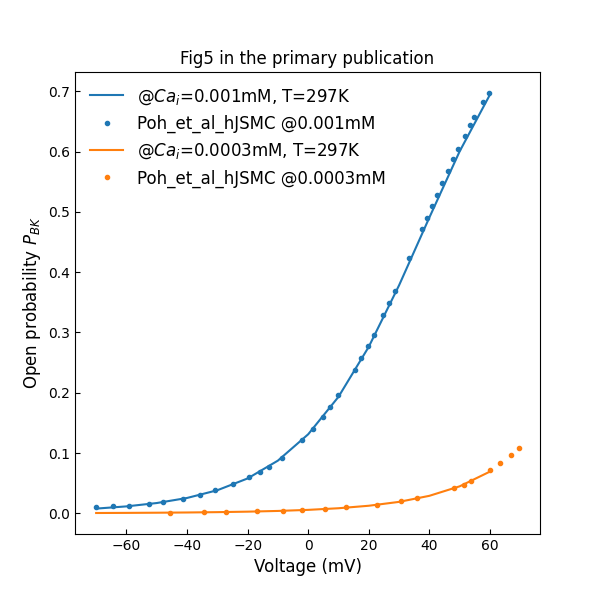
\includegraphics[width=\linewidth]{./figs/simFig5.png}
  \captionof{figure}{Open probability versus clamping voltage plots, across various free intracellular $Ca^{2+}$ concentrations  (\emph{c.f.,} Fig.~5 in \citet{poh2012quantitative}).}
  \label{simFig5}
\end{minipage}
\end{figure}


\autoref{simFig5} shows open probability of BK channel versus clamping voltage at various intracellular calcium concentrations.


\autoref{simFig6} shows normalized sodium channel peak I–V plot various intracellular $Na^+$ concentrations.

\begin{figure}
\centering
\begin{minipage}{.5\textwidth}
  \centering
  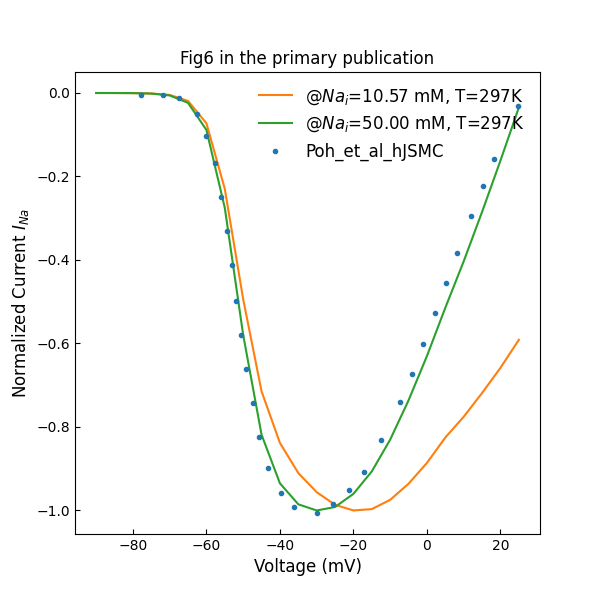
\includegraphics[width=\linewidth]{./figs/simFig6.png}
  \captionof{figure}{Normalized $Na^+$ channel peak I–V plot  (\emph{c.f.,} Fig.~6 in \citet{poh2012quantitative}).}
  \label{simFig6}
\end{minipage}%
\begin{minipage}{.5\textwidth}
  \centering
  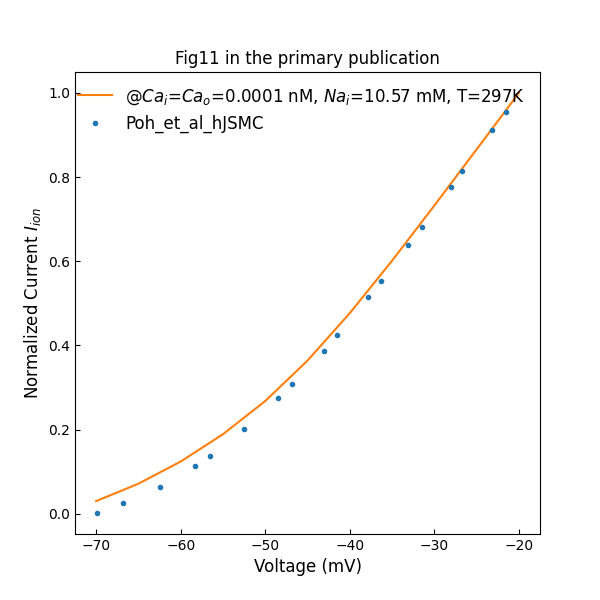
\includegraphics[width=\linewidth]{./figs/simFig11.png}
  \captionof{figure}{Simulated whole cell normalized I–V data under near calcium-free conditions  (\emph{c.f.,} Fig.~11 in \citet{poh2012quantitative}).}
  \label{simFig11}
\end{minipage}
\end{figure}

\autoref{simFig11} shows whole cell normalized I–V data from hJSMC model under near calcium-free conditions. The intracellular $Na^+$ concentration is set to 10.57 mM, while the value is unknown in the primary publication.

\subsection{Simulated action potentials}
In the \emph{periodic stimulation experiment}, the \emph{membrane potential component} is configured and parameterised with a periodic stimulus current. The parameters of stimulation can be changed and the following simulation uses 310 Kelvin for the temperature setting.

\autoref{simFig8} shows the simulated hJSMC action potential trace and free intracellular calcium concentration after a simulation of 30 minutes of electrical activity.

\begin{figure}[ht]\centering
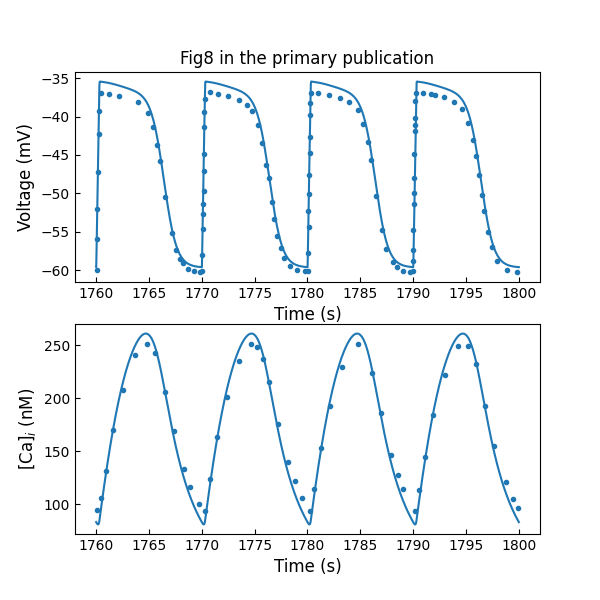
\includegraphics[width=0.7\linewidth]{./figs/simFig8.png}
\caption{simulated hJSMC action potential trace and free intracellular calcium concentration after a simulation of 30 minutes of electrical activity  (\emph{c.f.,} Fig.~8 in \citet{poh2012quantitative}).}
\label{simFig8}
\end{figure}


\subsection{Sensitivity Analysis}
In the \emph{sensitivity analysis experiment}, the \emph{membrane potential component} is configured to accept the changes of maximum conductance of ionic channels in the component \texttt{g\_parameters}.

\autoref{simFig13} shows sensitivity analysis by 50\% increase or decrease in maximum channel conductance. This evaluates the contributions of key ionic currents towards hJSMC membrane voltage. The last plot shows the free intracellular $Ca^{2+}$ concentrations corresponding to changes in $I_{CaL}$.

\begin{figure}[ht]\centering
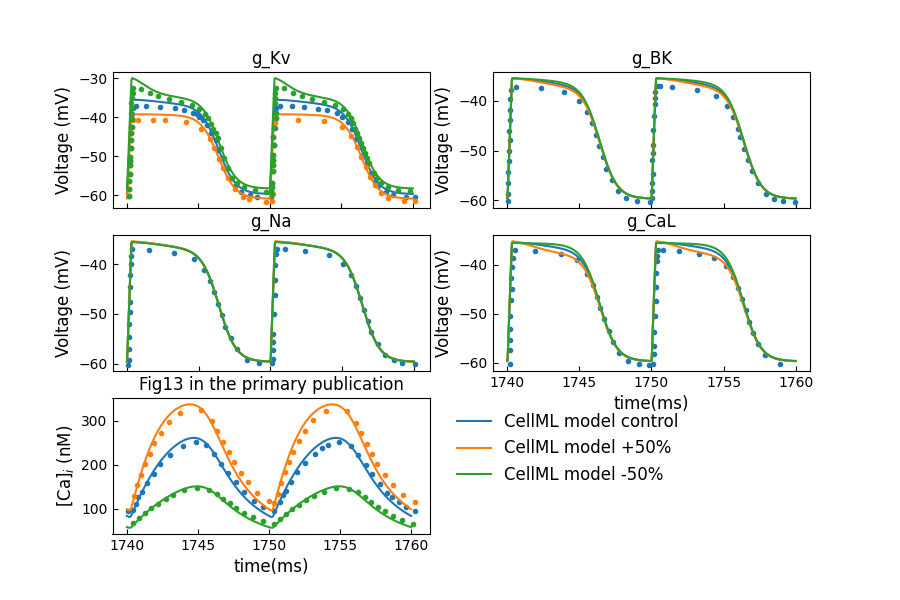
\includegraphics[width=0.9\linewidth]{./figs/simFig13.png}
\caption{Sensitivity analysis by 50\% increase or decrease in maximum channel conductance  (\emph{c.f.,} Fig.~13 in \citet{poh2012quantitative}).}
\label{simFig13}
\end{figure}

\section{Discussion}
\label{sec:discussion}

Based on the author provided model implementation \citep{poh2012quantitative}, we modularized the CellML implementation for reusability.
Additionally, we added clamped current component, patch clamp protocol and voltage clamp experiment to simulate ionic currents during a voltage clamp. We also modified the periodic current protocol and periodic stimulation experiment to enable the periodic stimulation for \autoref{simFig13}. 

During the curating process, we found some parameters (see \autoref{tab:parameters}) and equations (see \autoref{tab:equations}) which are inconsistent from the ones presented in the primary publication.

Since the clamping values for intracellular concentrations of $Ca_i^{2+}$ , $Na_i^+$ and $K_i^+$ were not specified in the paper, we used the initial values presented in the original CellML model in the first attempt. However, the difference becomes significant at less negative clamping voltages when reproducing the original Figures 2, 3, and 6. We then increased the intracellular concentrations for a better fit. However, the values of intracellular concentrations in particular $Ca_i^{2+}$ are quite larger than physiological value, which should be aware of in future usage of this model. 

\begin{table}[hbt!]\centering

\caption{Inconsistency of parameters}\label{tab:parameters}

\begin{tabular}{lccrr}
\toprule
Parameters & primary paper & Original CellML & C code & current CellML\\
\midrule
$P_{NaK}$ & 0.1852 & 9.26 & 16.197 & 16.197\\
$\tau_{dCat}$ & 1.9058 & 1.9058 & 1.9508 & 1.9508\\
1st factor in Eq(S-24) & 0.05956 & 0.05956 & 0.005956 & 0.005956\\
\bottomrule
\end{tabular}
\end{table}

\begin{table}[hbt!]\centering
\begin{threeparttable}
\caption{Inconsistency of equations}\label{tab:equations}

\begin{tabularx}{\textwidth} % {m{2cm}m{2cm}m{2.3cm}m{2.3cm}X}
\toprule
Equations & primary paper & Original CellML & C code & current CellML\\
\midrule
S-5, S-6, S-7 & without unit conversion & $\times 1e-15$ & $V_{cell}$ in $mm^3$ and $\times 1e-9$ & $\times 1e-15$\\
S-13, S-14 & No T\tnote{1} & with T\tnote{2} &  with T\tnote{2} & with T\tnote{2} and $T_{0}=310K$\\
S-23,..., S-28 & No T\tnote{1} & with T\tnote{2} &  with T\tnote{2} & with T\tnote{2} and $T_{0}=310K$\\
S-33, S-34& No T\tnote{1} & with T\tnote{2} &  with T\tnote{2} & with T\tnote{2} and $T_{0}=310K$\\
S-36, S-37,& No T\tnote{1} & with T\tnote{2} &  with T\tnote{2} & with T\tnote{2} and $T_{0}=297K$\\
S-43, S-44 & No T\tnote{1} & with T\tnote{2} &  with T\tnote{2} & with T\tnote{2} and $T_{0}=297K$\\
S-80,..., S-91& No T\tnote{1} & with T\tnote{2} &  with T\tnote{2} & with T\tnote{2} and $T_{0}=297K$\\
S-67,..., S-70& with $Ca_i^{2+}$ & without $Ca_i^{2+}$ & without $Ca_i^{2+}$ & without $Ca_i^{2+}$\\
S-75,..., S-78 & with $Ca_i^{2+}$ & without $Ca_i^{2+}$ & without $Ca_i^{2+}$ & without $Ca_i^{2+}$\\
\bottomrule
\end{tabularx}
\begin{tablenotes}
\item[1] No temperature correction.
\item[2] Multiplied by corresponding temperature factor $\phi=Q_{10}^{\frac{T-T_0}{10}}$.
\end{tablenotes}
\end{threeparttable}
\end{table}

\section*{Acknowledgements}
The authors gratefully acknowledge the assistance of Alberto Corrias and Martin Buist in the validation of the model implementation presented here.

\bibliography{sample}

\end{document}